\documentclass[final]{beamer}
\mode<presentation>{\usetheme{ParisSaclay}}
\usepackage[english]{babel}
\usepackage[utf8]{inputenc}
\usepackage[T1]{fontenc}
\usepackage{amsmath,amsthm,amssymb,latexsym}
\usepackage[orientation=portrait,size=a0,scale=1.4]{beamerposter}
\usepackage{graphicx}
\usepackage{tikz}
\usepackage{lipsum}
\usepackage{svg}

\boldmath

\title{\huge Research Poster Title}
\author{Author One \and Author Two \and Author Three}
\institute[]{Department Name, Faculty/School Name, The Hong Kong Polytechnic University}

\begin{document}

\begin{frame} [fragile]{} 

 
\begin{columns}[t]

    \begin{column}{.4\textwidth}
    \begin{block}{Overview}
    This poster template has been adapted for The Hong Kong Polytechnic University. Replace the placeholder text with your project summary, key claims, and contact details.

       \begin{itemize}
        \item Update the title, author list, department, and footer information.
        \item Put official logos and project graphics in the \texttt{assets} folder.
        \item Keep the PolyU maroon as the main accent color for visual consistency.
       \end{itemize}
   \end{block}
\vspace{1cm}
		\begin{alertblock}{Key Message}
			\[
                \text{Impact} = \frac{\text{Performance Gain} \times \text{Scalability}}{\text{Cost}}
            \]

			Use this space for the main takeaway that should be visible from a distance.
		\end{alertblock}
		
		\bigskip
		
	\begin{block}{Methodology}
	\begin{figure}
	\begin{tikzpicture}[scale=.95]
		\draw [domain=0:29,samples=50,ultra thick,rouge] plot [mark=*,mark size=5] (\x,{18-18/((\x/3)^2+1)});
		\draw (0,0)rectangle(30,20) ;
		\foreach \o in {0,2,...,20} \draw(-1,\o)node[left]{\o};
		\foreach \a in {0,1,...,15} \draw(\a*2,0)node[below]{\a};

	\end{tikzpicture}
	\caption{Example chart for experimental or simulation results.}
	\end{figure}
	\lipsum[1][1-2]
	\end{block}
	\vspace{1cm}
	\begin{block}{Results}
	\begin{figure}
	\begin{tikzpicture}[scale=2]
		\fill [black] (0,-4) rectangle (10,4);
		\draw [very thin, gray] (0,-4) grid (10,4);
		\draw [domain=0:10,samples=200,ultra thick,vertl] plot (\x,{2*sin(\x*60)+sin(\x*720)/2});
		\draw [domain=0:10,samples=100,thick,mandarine] plot (\x,{2*sin(\x*60-30)});
	\end{tikzpicture}
	\caption{Example comparison between baseline and proposed method.}
	\end{figure}
	 \lipsum[1][3-4]
	\end{block}
	  
	\end{column}
	
% ---------------------------------------------------------%

    \begin{column}{.4\textwidth}	
	\begin{exampleblock}{Research Highlights}
	\lipsum[3]
	\end{exampleblock}
	
\vspace{1cm}		
	
	\begin{block}{Visual Abstract}
	\begin{figure}
	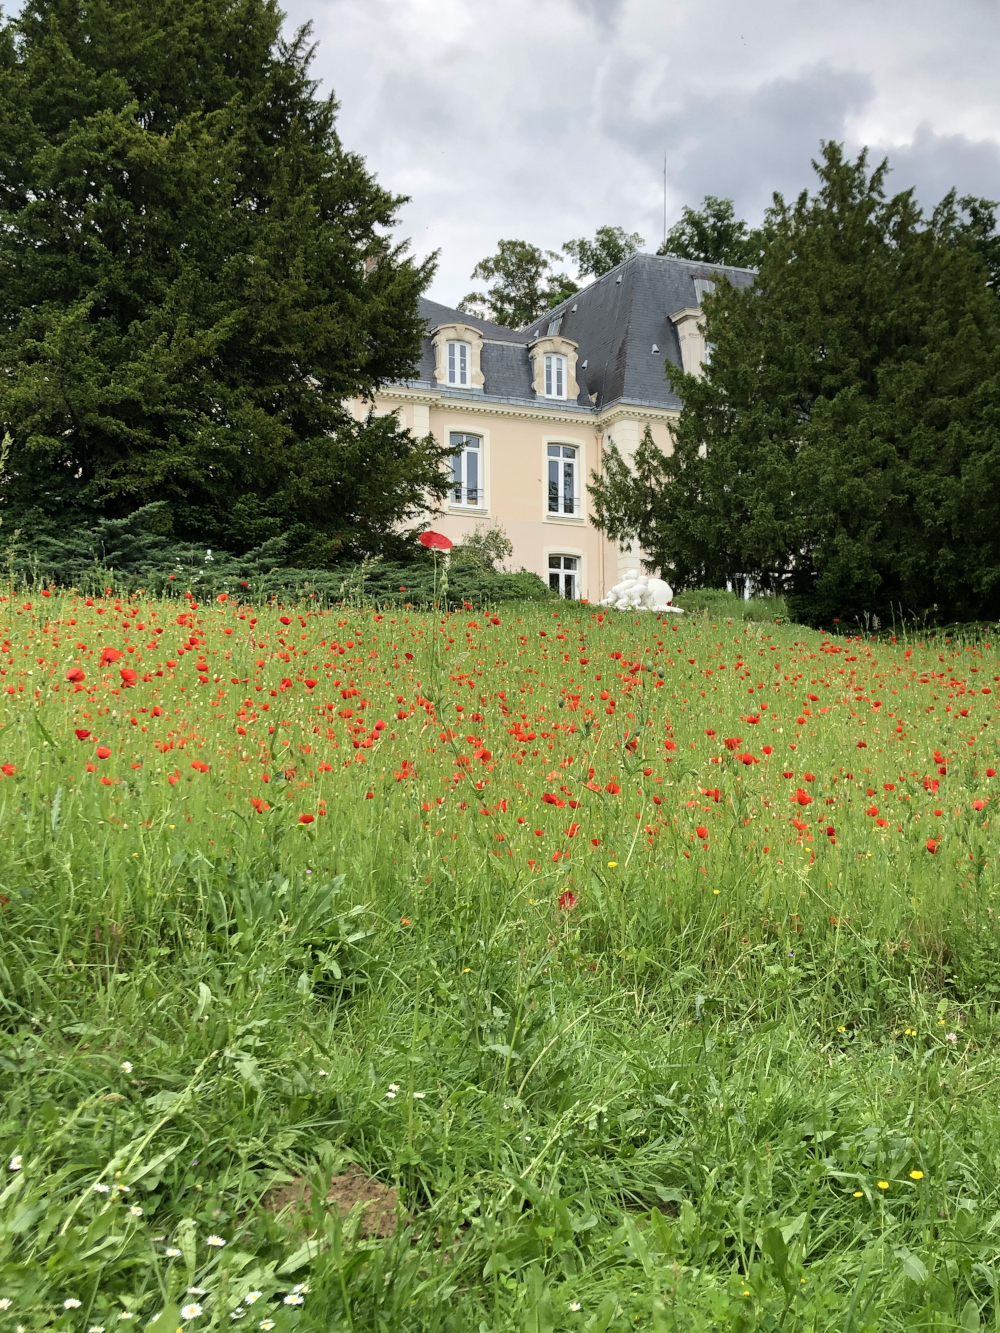
\includegraphics[width=.9\textwidth]{300} 	
	\caption{Replace with a schematic, pipeline, or representative result.}
	
	\end{figure}
	
	\lipsum [4][1-4]
	\end{block}
	
	\vspace{1cm}	

		\begin{exampleblock}{References}
			\begin{enumerate}
       			\item First reference in your preferred citation format.
       			\item Second reference for a core method, dataset, or theory.
       			\item Third reference for a benchmark or prior result.
       		\end{enumerate}

\vspace{1cm}		
		
		\end{exampleblock}
		
		\begin{exampleblock}{Acknowledgements}
			Supported by your grant, laboratory, industry partner, or PolyU internal funding scheme.
		
		\end{exampleblock}

	\end{column}
\end{columns}




    
\end{frame}

\end{document}
